\documentclass[class=book, crop=false, oneside, 12pt]{standalone}
\usepackage{standalone}
\usepackage{../../style}
\usepackage[normalem]{ulem}
\graphicspath{{./assets/images/}}

% arara: pdflatex: { synctex: yes, shell: yes }
% arara: latexmk: { clean: partial }
\begin{document}
\part{Aftermath}
\chapter{La generazione del codice intermedio}
\section{Riepilogo sulla fase frontend della compilazione}
Durante il nostro percorso abbiamo avuto modo di attraversare quasi tutte le fasi che costituiscono il cosiddetto \emph{frontend} della compilazione:
\begin{itemize}
    \item l'analisi lessicale ha il compito di distinguere i vari lessemi in un dato input e successivamente restituire una stringa di tokens, ossia di elementi che possono essere correttamente letti da un analizzatore sintattico; inoltre, ha il compito di iniziare a popolare la tabella dei simboli;
    \item l'analisi sintattica, su cui non ci dilunghiamo troppo in questa sede dal momento che costituisce circa \(\frac{1}{3}\) di questo elaborato già da sola, verifica se la stringa ottenuta dall'analisi lessicale appartiene al linguaggio di una data grammatica (restituendo in caso positivo l'albero di derivazione); è interessante specificare che, in molti casi, a questa fase vengono accorpate ulteriori operazioni, come ad esempio la stessa analisi semantica;
    \item l'analisi semantica, che si occupa di fare controlli statici, ad esempio circa la compatibilità di operandi e operatori nei vari statements (è qui che si scoprono errori come tentativi di somma tra un \texttt{int} e un \texttt{float} o tentativi di conversione di tipo quando si fa uso di un operatore che consente operazioni tra tipi misti), o anche altri riguardanti la validità di istruzioni condizionali e di controllo (\texttt{if}, \texttt{while} e \texttt{break}).
\end{itemize}
A valle di tutto questo troviamo l'ultima fase del frontend della compilazione, la generazione del codice intermedio; al pari dell'analisi semantica, è possibile che anche quest'ultima fase venga implementata come parte integrante dell'analisi sintattica, e in particolare ci sono degli schemi di traduzione che vanno a sfruttare gli alberi di sintassi astratta (AST) che abbiamo visto quando abbiamo parlato di analisi semantica.

\section{Il codice intermedio}
Il codice  intermedio è una rappresentazione del nostro codice di partenza, abbastanza astratta da nascondere alcune specifiche che sono tipiche del codice macchina e che ne rendono la lettura poco agevole (come ad esempio i movimenti di informazioni tra registri o tra memoria e registri), ma comunque più specifica del linguaggio originale da cui siamo partiti.

\subsection{Rappresentazione del codice intermedio}
Non abbiamo una sola possibilità per rappresentare il codice intermedio; a seguito presenteremo quelle più comunemente utilizzate.

\paragraph{Strutture a grafo}
Una prima via è quella di utilizzare delle strutture a grafo partendo dai parse trees, come ad esempio gli stessi AST o dei grafi diretti aciclici (DAG). Questi ultimi sono spesso più succinti degli AST: immaginiamo che un AST abbia due foglie con uno stesso identificatore \(a\): in un DAG avremmo lo stesso nodo con più archi entranti. Gli AST sono a loro volta più succinti dei parse trees: questi spesso devono ricorrere a cammini molto lunghi per rappresentare certe derivazioni, rallentando di molto le operazioni che ci troveremo a fare in seguito.

\paragraph{Codice a tre indirizzi}
Una possibilità, leggermente migliore, è anche quella di utilizzare il cosiddetto \emph{codice a tre indirizzi}, così chiamato perché non prevede la possibilità di referenziare più di tre valori in un singolo statement (che quindi avrà forma \texttt{x = y op z}), limitando enormemente la complessità degli stessi.

\paragraph{Codice in un altro linguaggio}
Una terza strada percorribile è quella di utilizzare un altro linguaggio di programmazione come vero e proprio codice intermedio. Questo approccio ci risparmia inoltre il problema di implementare da noi un backend per la compilazione, perché da questo momento in poi possiamo tranquillamente utilizzare la catena di compilazione del linguaggio che stiamo usando come codice intermedio. In questi casi la scelta favorita è il C, perché è un linguaggio incredibilmente flessibile e dispone dell'eccellente compilatore \texttt{gcc}.

\subsection{Il codice a tre indirizzi}
In un certo senso, il codice a tre indirizzi è una rappresentazione testuale di un AST. Per capire di cosa stiamo parlando, è utile andare subito a vedere un esempio di traduzione da AST a codice a tre indirizzi. Consideriamo il seguente AST:
\begin{figure}[H]
    \centering
    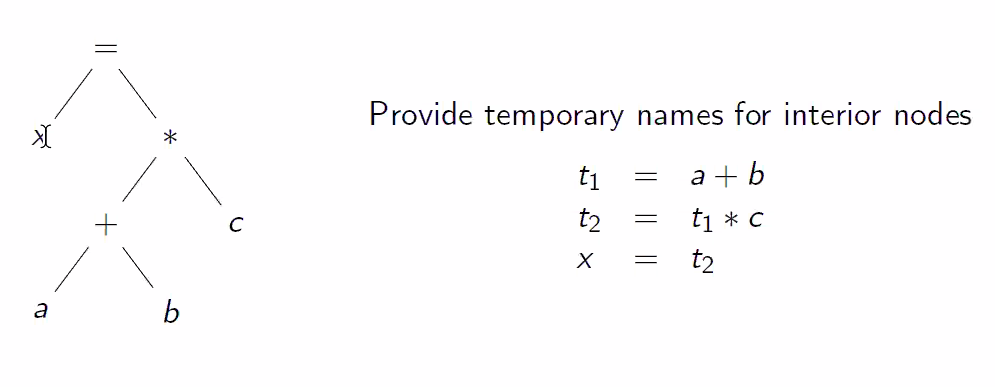
\includegraphics[width=.8\textwidth]{ex1.png}
    \caption{AST per l'espressione \texttt{x = (a + b) * c}}
    \label{fig:ast-to-tac-ex1}
\end{figure}
In questo caso abbiamo l'AST per una banale espressione aritmetica (con un minimo di parentesizzazione), abbastanza semplice da ricostruire partendo dalle foglie dei livelli più bassi. L'equivalente rappresentazione dell'AST nel codice a tre indirizzi può essere ottenuta salvando l'esito delle operazione intermedie in dei registri temporanei, come segue:
\begin{align*}
    t_1 &= a + b \\
    t_2 &= t_1 * c \\
    x &= t_2
\end{align*}
Avere una rappresentazione testuale di un AST, facendo uso del codice a tre indirizzi, è comodo perché semplifica la generazione di linguaggio macchina e la sua ottimizzazione; tuttavia questa tecnica non è molto frequente, perché è dipendente dalla macchina per cui stiamo scrivendo il backend (machine dependent).

\subsection{Esempio di generazione del codice intermedio}
Supponiamo di partire con un'espressione come questa\footnote{Originariamente l'espressione era stata scritta come \(\textrm{\texttt{if (x < 100 || x > 200 \&\& x != y) x = 0;}}\), ma noi abbiamo deciso di aggiungere quelle parentesi perché è così che è stata effettivamente valutata nella traduzione, almeno se applichiamo il corretto ordine di precedenza degli operatori logici (\(\textrm{\texttt{\&\&}} \preceq \textrm{\texttt{||}}\)).}:
\begin{equation*}
    \textrm{\texttt{if ((x < 100) || (x > 200 \&\& x != y)) x = 0;}}
\end{equation*}
Una prima approssimazione di codice intermedio che possiamo ottenere è questa:
\begin{minted}{asm}
    if x < 100 goto L2
    goto L3
L3: if x > 200 goto L4
    goto L1
L4: if x!= y goto L2
    goto L1
L2: x = 0
L1:
\end{minted}
Possiamo osservare come in questa traduzione siano state sfruttate le regole di cortocircuitazione: se infatti \texttt{x < 100} viene valutata come vera, allora si esce subito dal controllo. Tuttavia, in quella traduzione abbiamo numerosi \texttt{goto} ridondanti; ci permettiamo dunque di presentare una traduzione leggermente migliore:
\begin{minted}{asm}
    if x < 100 goto L2
    iffalse x > 200 goto L1
    iffalse x!= y goto L1   
L2: x = 0
L1:
\end{minted}
il controllo sulla falsità di \texttt{x} ci permette di ridurre il numero di righe e labels utilizzate, nonché sfruttare meglio la corticircuitazione, caratteristica fondamentale per un buon compilatore. Si tenga sempre a mente che non sempre le condizioni vengono valutate nello stesso esatto ordine in cui sono state scritte dal programmatore.

\section{Statement per il controllo di flusso}
A questo punto possiamo andare a vedere più da vicino la traduzione in codice intermedio di alcuni statements. In particolare ci interessano i seguenti:
\begin{align*}
    P &\to S \\
    S &\to if (B) S_1 \\
    S &\to while (B) S_1 \\
    &\ldots \\
    B &\to \textrm{\texttt{true}} \\
    B &\to \textrm{\texttt{false}} \\
    B &\to B_1\; ||\; B_2 \\
    B &\to B_1\; \&\&\; B_2
\end{align*}
In questo schema \(P\) sta per \emph{program}, \(S\) sta per \emph{statement} e \(B\) sta per \emph{boolean}.

\subsection{Istruzioni condizionali}
Diamo un'occhiata alla generazione del codice intermedio di un'istruzione condizionale come potrebbe essere un comune costrutto \texttt{if-then}. Possiamo schematizzarne la struttura in questo modo:
\begin{figure}[H]
    \centering
    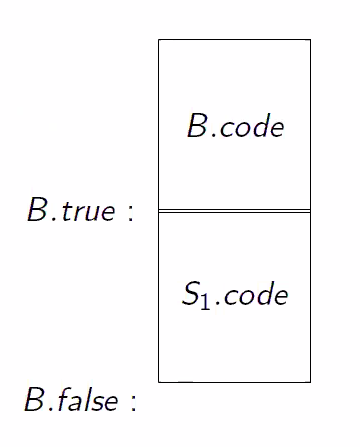
\includegraphics[width=.3\textwidth]{if-then-abstract.png}
    \caption{}
    \label{}
\end{figure}
dove l'etichetta \(B.true\) punta al body dell'istruzione condizionale (perché naturalmente vuol dire che la condizione è stata verificata), mentre l'etichetta \(B.false\) punta alla prima istruzione successiva alla chiusura del blocco \texttt{then}.

\paragraph{Attributi}
Andiamo a vedere di preciso quali attributi abbiamo in questo processo:
\begin{itemize}
    \item \(S.next\), attributo ereditato: ci dice qual è la posizione della primissima istruzione da eseguire dopo aver concluso l'esecuzione del blocco di codice \(S\); conservare l'etichetta è utile, perché \(S\) potrebbe avere degli altri statements di controllo annidati (ad esempio un ciclo \texttt{while} o una catena di \texttt{if}), per cui è importante poter sempre sapere qual è l'istruzione che deve essere eseguita dopo lo statement padre;
    \item \(S.code\), attributo sintetizzato: è il codice intermedio che implementa lo statement che stiamo considerando; termina con un istruzione di salto a \(S.next\);
    \item \(B.true\), attributo ereditato: questa etichetta punta alla prima istruzione da eseguire se la condizione di \(B\) risulta vera;
    \item \(B.false\), attributo ereditato: per analogia a \(B.true\), questo attributo punta alla prima istruzione da eseguire nel caso in cui \(B\) sia valutato come falso;
    \item \(B.code\), attributo ereditato per gli statements, sintetizzato se guardiamo solo l'SDD delle condizioni booleane: è la sequenza dei passi di codice intermedio che implementano la condizione booleana e determinano se passare a \(B.true\) o \(B.false\).
\end{itemize}

\paragraph{Nota sui booleani}
In questo è bene puntualizzare un distinguo sui due diversi ruoli che possono assumere i booleani:
\begin{itemize}
    \item alterare il flusso di esecuzione, e quindi operare come \emph{condizioni booleane};
    \item calcolare il valore di espressioni logiche, e quindi comportarsi come \emph{espressioni booleane} (e quindi come r-values).
\end{itemize}
Quella che noi consideriamo oggi è la prima funzione; nel secondo caso si comportano esattamente come delle normali espressioni aritmetiche, che lavorano con valori e operatori logici anziché numerici. Molto spesso le grammatiche si trovano ad avere non-terminali diversi per questi due ruoli.

\subsection{Il programma come statement}
Andiamo ora a vedere da vicino la prima istruzione dalla nostra lista, \(P \to S\); ne approfitteremo per dare un'occhiata anche a quale tipo di notazioni e regole di sintassi (più o meno) utilizzeremo in questo processo.
\begin{align*}
    P &\to S & S.next &= newlabel() \\
    & & P.code &= S.code \triangleright label(S.next)
\end{align*}
Il senso stesso dell'espressione \(P \to S\) sembra suggerire che il programma \(P\) possa essere visto globalmente come uno statement.
\begin{itemize}
    \item \(newlabel()\) è una funzione che, una volta invocata, genera una nuova etichetta;
    \item \(\triangleright\) è un opereatore che denota la concatezione di due (o più) segmenti di codice intermedio;
    \item \(label(L)\) assegna l'etichetta \(L\) alla prossima istruzione a tre indirizzi generata;
    \item \(S.next\), come intuibile, è l'etichetta che denota la prima istruzione da eseguire dopo la fine di \(S\); se ipoteticamente volessimo uscire da \(S\) prima della chiamata a \(S.next\), allora dovremmo esplicitamente eseguire un \texttt{goto}.
\end{itemize}
Inoltre possiamo vedere come l'attributo sintetizzato \(P.code\) venga definito con l'ausilio dell'operatore \(\triangleright\).

\subsection{Semplice blocco \texttt{if-then}}
Vediamo adesso nello specifico come tradurre uno statement \(S\) che si compone di un'istruzione di \texttt{if-then} semplice, senza un blocco \texttt{else}.
\begin{align*}
    S &\to if (B) S_1 & B.true &= newlabel() \\
    & & B.false &= S_1.next = S.next \\
    & & S.code &= B.code \triangleright label(B.true) \triangleright S_1.code
\end{align*}
La prima cosa che facciamo è creare una nuova label \(B.true\) che etichetti l'inizio del blocco di codice da eseguire nel caso in cui la condizione \(B\) sia verificata. Nel caso in cui \(B\) risulti invece falsa, assegnamo all'etichetta di \(B.false\) il blocco successivo ad \(S_1\) (quindi successivo al blocco \texttt{then}); dal momento che in questo caso non abbiamo anche un \texttt{else}, il codice successivo a \(S_1\) sarà quello successivo a tutto lo statement \(S\).

Complessivamente, il valore che assegnamo al nostro statement \(S\) sarà quindi costituito dal codice della condizione booleana \(B.code\), l'etichetta \(B.true\) e il blocco di codice da eseguire nel caso in cui l'istruzione sia verificata (\(S_1.code\)). Nel caso in cui la condizione booleana non fosse valutata come vera, il programma eseguirebbe, come detto in precedenza, la prima istruzione contenuta in \(B.false\). 

\subsection{Blocco \texttt{if-then-else}}
Supponiamo di voler tradurre un'istruzione condizionale che comprende anche un blocco \texttt{else}. Questo naturalmente cambia leggermente la traduzione, poiché l'etichetta \(B.false\) non punterà più alla prima istruzione successiva al blocco \texttt{then}, bensì dovrà essere creata ex novo, e punterà alla prima istruzione del blocco \texttt{else}.
\begin{figure}[H]
    \centering
    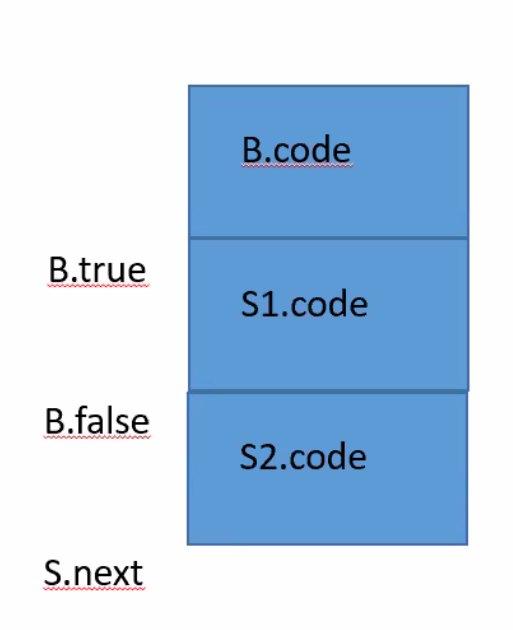
\includegraphics[width=.4\textwidth]{if-else-trans.png}
    \caption{}
    \label{}
\end{figure}
Entrambe le etichette \(S_1.next\) e \(S_2.next\) punteranno all'istruzione successiva all'intero statement.
\begin{align*}
    S &\to if (B) S_1 else S_2 & B.false =\; &newlabel() \\
    & & B.true =\; &newlabel() \\
    & & S_1.next =\; &S.next \\
    & & S_2.next =\; &S.next \\
    & & S.code =\; &B.code \triangleright label(B.true) \triangleright S_1.code\; \triangleright \\
    & & &gen(goto\; S.next) \triangleright label(B.false) \triangleright S_2.code
\end{align*}
Il codice intermedio dello statement \(S\) è dato quindi dalla concatenazione di tutti questi blocchi; particolare riguardo all'istruzione \(gen(goto\; S.next)\), che deve essere eplicitata per poter saltare all'istruzione contenuta in \(S.next\).

\subsection{Traduzione di un ciclo \texttt{while}}
Prendiamo adesso visione del codice intermedio di un ciclo. 
\begin{itemize}
    \item La prima cosa che facciamo è assegnare due \(newlabels()\): una la chiameremo \(begin\), e punterà all'inizio del ciclo (quindi all'espressione \(B.code\)); l'altra \(B.true\), e indicherà l'inizio del corpo del ciclo \(S_1\) e a cui andiamo quindi in caso l'espressione contenuta in \(B.code\) sia verificata.
    \item Nelle istruzioni condizionali viste prima ci siamo abituati ad vedere \(S_1.next\) puntare a \(S.next\), poiché al termine del corpo di un'istruzione condizionale normalmente proseguiamo con l'esecuzione del codice; in questo caso, invece, al termine del corpo dell'istruzione dovremmo tornare ad eseguire il controllo \(B.code\) e, eventualmente, rieseguire il corpo del ciclo stesso, per cui \(S_1.next\) dovrà puntare a \(begin\).
\end{itemize}
A questo punto, la composizione dell'attributo sintetizzato \(S.code\) dovrebbe seguire naturalmente.
\begin{align*}
    S &\to while (B) S_1 & begin =\; &newlabel() \\
    & & B.true =\; &newlabel() \\
    & & B.false =\; &S.next \\
    & & S_1.next =\; &begin \\
    & & S.code =\; &label(begin) \triangleright B.code \triangleright label(B.true)\; \triangleright \\
    & & &S_1.code \triangleright gen(goto\; begin)
\end{align*}

\subsection{Traduzione di operazioni booleane}
Per concludere, diamo un'occhiata rapida alla traduzione delle espressioni logiche. Lo faremo andando a confrontare la diversa traduzione di due semplici operazioni di \texttt{OR} e \texttt{AND}:
\begin{align*}
    B &\to B_1\; ||\; B_2 & B &\to B_1\; \&\&\; B_2 
\end{align*}
Andiamo a confrontare il codice intermedio di queste due espressioni, riga per riga, in modo da apprezzarne le analogie e il modo in cui sfruttano la cortocircuitazione:
\begin{itemize}
    \item l'etichetta \(B_1.true\) rimanda direttamente all'etichetta \(B.true\) dell'intero statement nel caso dell'\texttt{OR} (perché naturalmente è sufficiente che un elemento sia \(true\) per rendere valida l'intera espressione), mentre invece per \texttt{AND} viene semplicemente creata una nuova label;
    \item la situazione è assolutamente analoga, ma a parti invertite, per l'etichetta \(B_1.false\);
    \item nelle due righe successive andiamo a definire le etichette per il secondo elemento delle nsotre espressioni e, in entrambi i casi, queste ultime punteranno alle etichette di uscita dell'intero statement; questo accade perché sono l'ultimo elemento dell'espressione ed il loro valore andrà a determinare quello dell'intera espressione;
    \item la differenza nella composizione di \(B.code\) sta quindi esclusivamente nell'etichetta che si frappone fra il codice del primo e del secondo elemento: nel caso dell'\texttt{OR}, infatti, il secondo elemento verrà valutato solo se il primo risulta falso (e qui infatti mettiamo la nuova etichetta \(B_1.false\)); viceversa nell'\texttt{AND} valutiamo il secondo solo se il primo è vero, e quindi l'etichetta frapposta è \(B_2.false\).
\end{itemize}
\begin{align*}
    &B_1.true &=\; &B.true & &B_1.true &=\; &newlabel() \\
    &B_1.false &=\; &newlabel() & &B_1.false &=\; &B.false \\
    &B_2.true &=\; &B.true & &B_2.true &=\; &B.true \\
    &B_2.false &=\; &B.false & &B_2.false &=\; &B.false \\
    &B.code &=\; &B_1.code\; \triangleright & &B.code &=\; &B_1.code\; \triangleright \\
    &&&label(B_1.false) \triangleright  B_2.code & &&&  label(B_1.true) \triangleright B_2.code
\end{align*}

\section*{Una precisazione}
Se a questo punto avete l'impressione che tutto questo capitolo sia molto sconnesso e senza una conclusione (o in realtà del vero e proprio contenuto)... beh, sappiate che è la stessa sensazione che ha provato l'autore. 

Tutta la squadra ha avuto l'impressione che l'argomento non sia stato per nulla approfondito e in realtà abbiamo il sospetto che la professoressa sia una grande fan di Speedy Gonzales, ma... Hey, questo è quello che passa il convento e pare che questi argomenti nemmeno siano presenti all'esame. Mai dire mai però, quindi occhi aperti e guardia alta.

\end{document}
